% =====================================================================
% Laporan Tugas - Workshop Deep Learning (Teknik Telekomunikasi ITERA)
% Studi Ablasi RNN, LSTM, GRU vs ANN untuk Prediksi Trafik Seluler
% Compile: pdflatex main && bibtex main && pdflatex main && pdflatex main
% =====================================================================
\documentclass[conference,a4paper]{IEEEtran}
\IEEEoverridecommandlockouts

\usepackage[indonesian]{babel}
\usepackage[utf8]{inputenc}
\usepackage[T1]{fontenc}
\usepackage{cite}
\usepackage{amsmath,amssymb}
\usepackage{graphicx}
\usepackage{booktabs}
\usepackage{siunitx}
\usepackage{xcolor}
\usepackage{subcaption}
\usepackage{url}
\captionsetup{font=footnotesize}
\graphicspath{{gambar/}}

\begin{document}

\title{Studi Ablasi RNN, LSTM, dan GRU dibandingkan\\ANN untuk Prediksi Trafik Seluler Kota Milan}

\author{
\IEEEauthorblockN{Ade Raka Maulana}
\IEEEauthorblockA{NIM 124400047\\Teknik Telekomunikasi, ITERA\\ade.124400047@student.itera.ac.id}
}

\maketitle

\begin{abstract}
Laporan ini menelaah faktor apa saja yang paling memengaruhi akurasi prediksi trafik internet per jam pada empat arsitektur: ANN, RNN, LSTM, dan GRU. Data berasal dari dataset Telecom Italia Big Data Challenge, dengan lokasi utama kotak Duomo (5060) dan lokasi kelompok Universitas Bicocca. Kami mengablasi lima faktor wajib (panjang jendela, ukuran hidden, jumlah lapisan, \emph{learning rate}, kelompok fitur) dan empat faktor pilihan (\emph{batch size}, \emph{dropout}, fungsi \emph{loss}, \emph{patience}), masing-masing dengan tiga seed (total 420 run). Temuan utama: GRU dan RNN paling akurat di Duomo dengan MAE uji sekitar 222 dan 226, atau sekitar 52\% lebih rendah daripada baseline naif terbaik (468); ANN paling sensitif terhadap panjang jendela dan \emph{dropout}; LSTM paling rentan terhadap penambahan lapisan; serta \emph{learning rate} 0,0001 membuat semua model belum konvergen dalam 300 epoch. Di Bicocca, yang polanya tidak stasioner, konfigurasi terbaik dari Duomo tetap memperbaiki ANN, LSTM, dan GRU pada pekan uji, urutan model berubah, dan pada pekan Natal baseline naif sederhana mengalahkan semua model.
\end{abstract}

\begin{IEEEkeywords}
prediksi trafik seluler, RNN, LSTM, GRU, studi ablasi
\end{IEEEkeywords}

\section{Pendahuluan}
Operator seluler perlu meramal trafik per sel untuk mengatur kapasitas dan menghemat energi jaringan. Model sekuensial seperti RNN, LSTM, dan GRU banyak dipakai untuk peramalan deret waktu \cite{lim2021} dan telah diterapkan pada trafik seluler \cite{jaffry2020,santos2022}, karena membawa keadaan tersembunyi dari satu jam ke jam berikutnya, sedangkan ANN hanya melihat jendela masukan sebagai satu vektor datar. Pendekatan yang lebih rumit, misalnya \emph{federated learning} berbasis \emph{dual attention} \cite{zhang2021}, juga dikembangkan. Namun data per jam pada satu kota dan hanya beberapa minggu latih relatif kecil, sehingga belum jelas apakah model yang lebih kompleks selalu lebih baik. Karena itu kami tidak hanya membandingkan keempat model, tetapi menanyakan hiperparameter mana yang benar-benar berpengaruh melalui studi ablasi, yaitu mengubah satu faktor sambil menahan faktor lain pada konfigurasi acuan.

Kontribusi laporan ini adalah (i) studi ablasi terkontrol dengan tiga seed per konfigurasi yang melaporkan rata-rata dan simpangan baku, (ii) perbandingan terhadap tiga baseline naif, (iii) pemilihan konfigurasi terbaik per model berdasarkan MAE validasi, dan (iv) uji generalisasi ke lokasi lain, yaitu Universitas Bicocca.

\section{Data dan Metode}
\subsection{Dataset}
Kami memakai Telecom Italia Big Data Challenge versi agregat per jam untuk wilayah Milan, yang juga dipakai pada penelitian prediksi trafik seluler sebelumnya \cite{jaffry2020,santos2022}, dengan periode November--Desember 2013. Fitur yang tersedia ialah aktivitas internet (\texttt{net}), panggilan (\texttt{call}), SMS (\texttt{sms}), serta jam dan hari dalam pekan yang diturunkan dari indeks waktu. Lokasi utama adalah kotak Duomo (5060); lokasi tugas kelompok adalah Universitas Bicocca (kode lokasi 7). Gambar~\ref{fig:peta} menunjukkan letak lokasi-lokasi tugas pada peta Milan. Gambar~\ref{fig:pola} memperlihatkan bahwa Duomo memiliki pola harian dan mingguan yang stabil dengan puncak sekitar 6.000--9.000, sedangkan aktivitas Bicocca turun tajam dari puncak sekitar 5.000 pada awal November menjadi sekitar 2.000 mulai akhir November dan hanya sekitar 200 menjelang akhir Desember.

\begin{figure}[t]
\centering
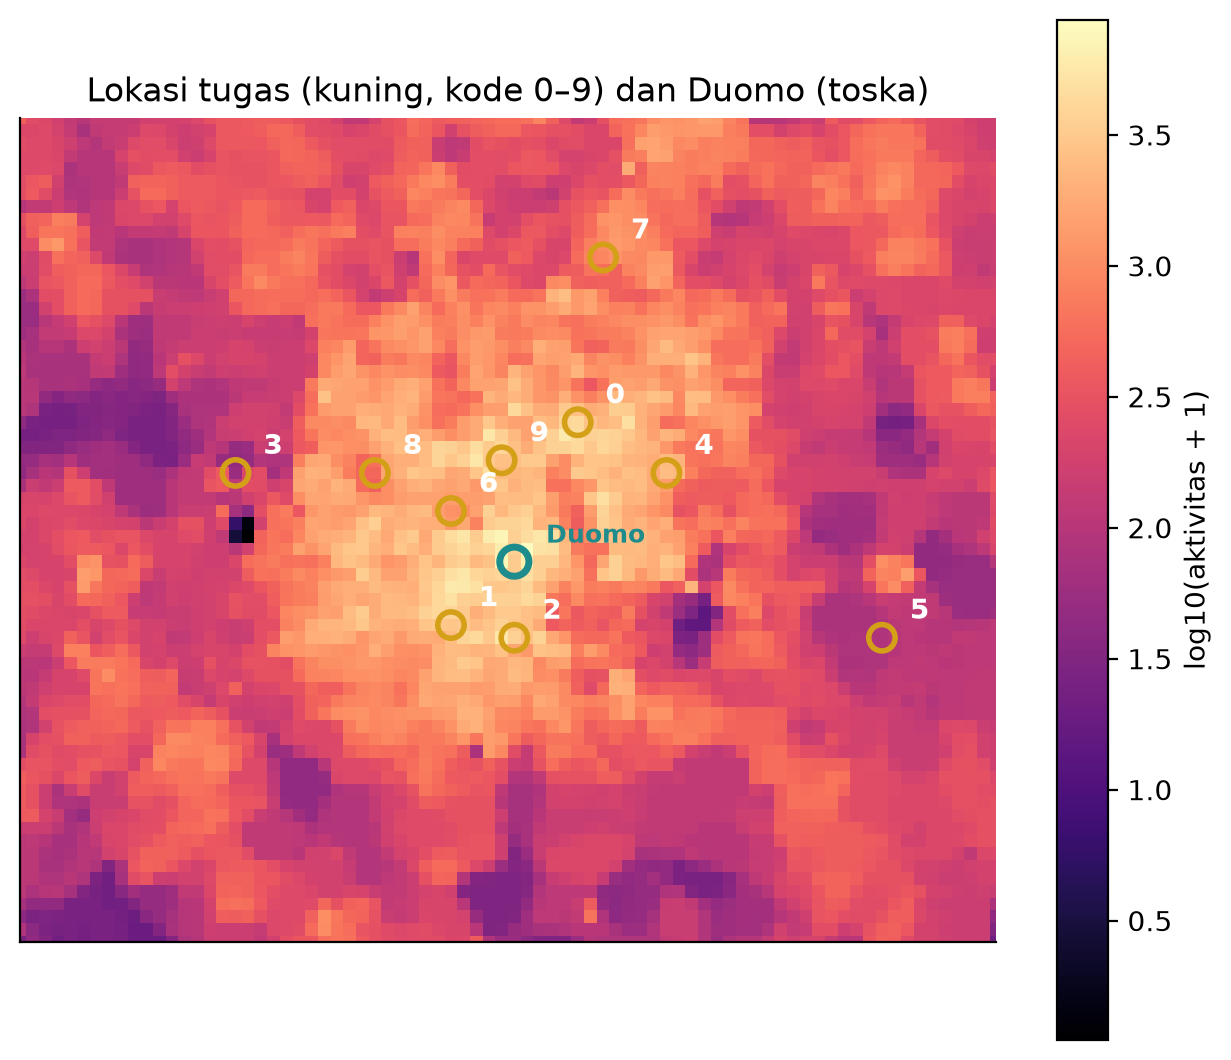
\includegraphics[width=\columnwidth]{peta_lokasi_tugas.png}
\caption{Rata-rata aktivitas internet per kotak di Milan dan lokasi-lokasi tugas.}
\label{fig:peta}
\end{figure}

\begin{figure}[t]
\centering
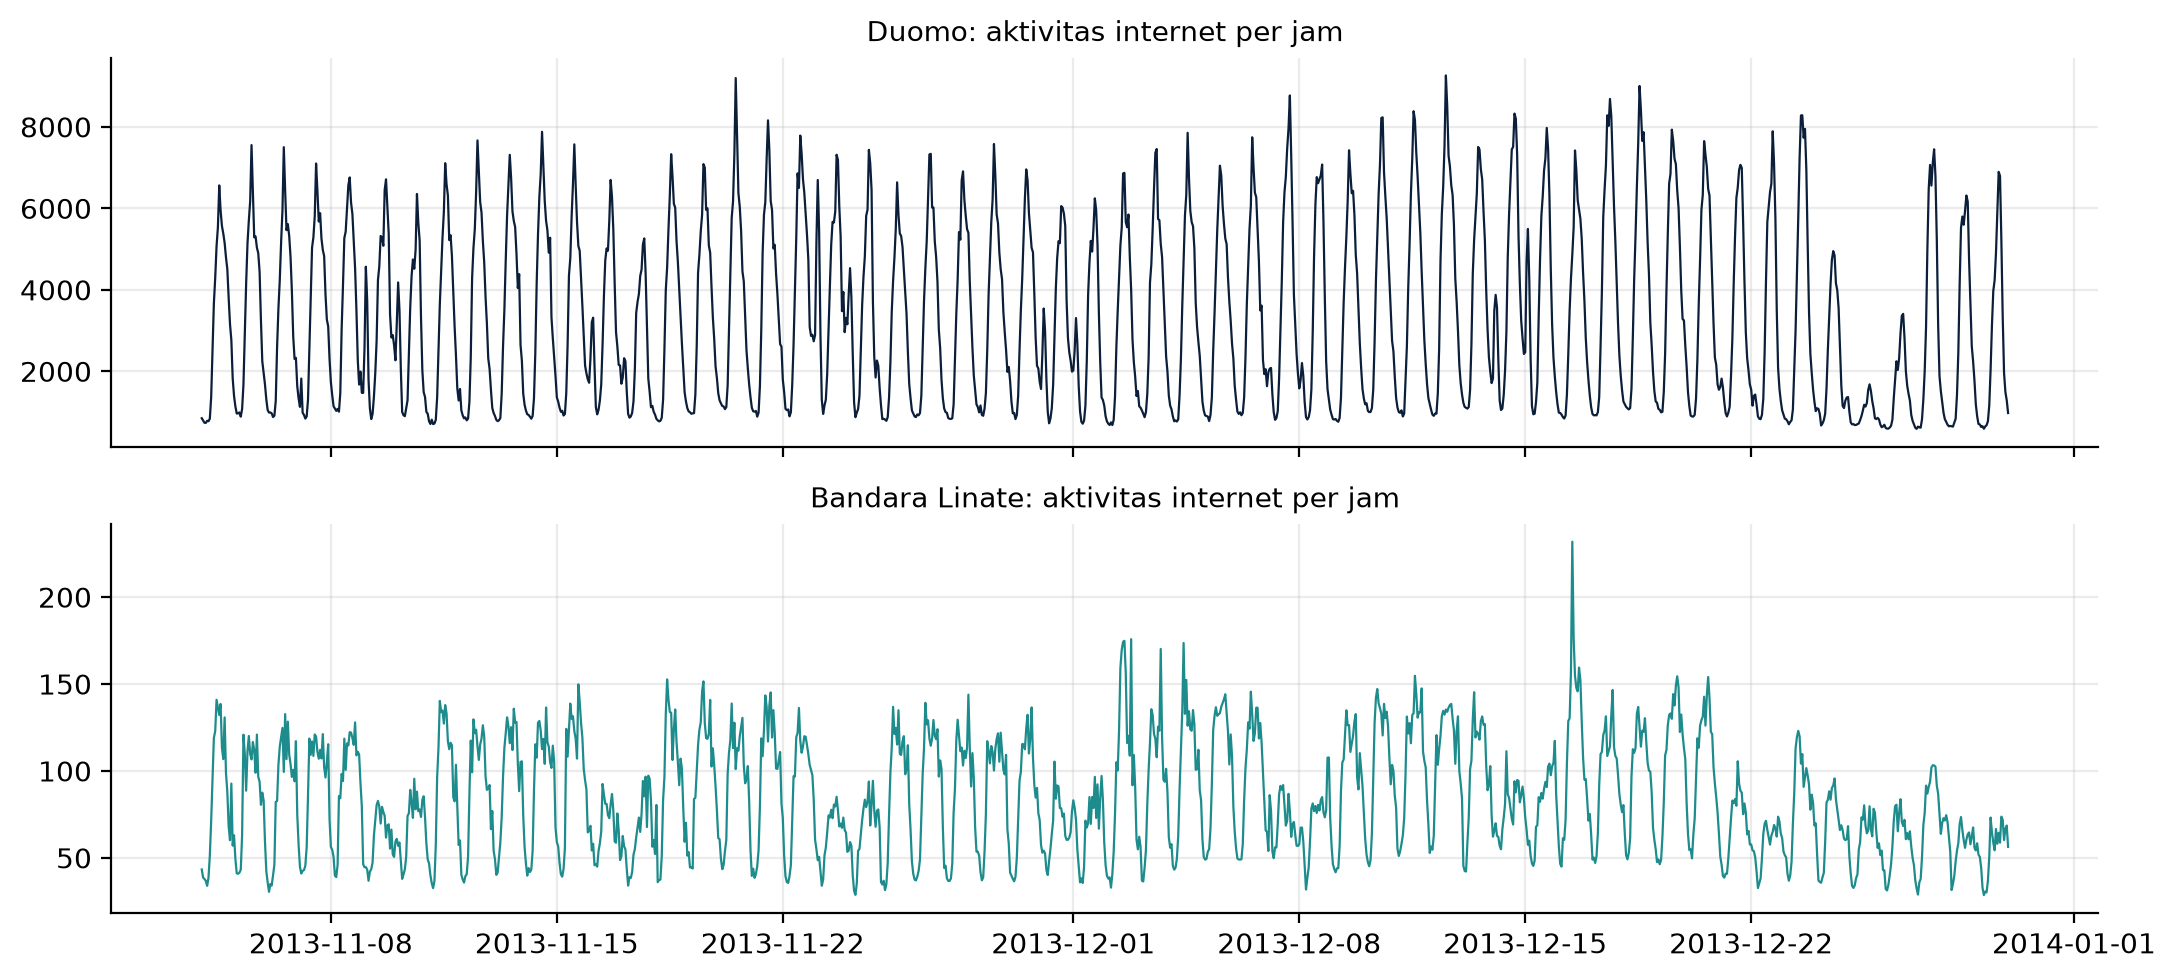
\includegraphics[width=\columnwidth]{D_pola_lokasi.png}
\caption{Aktivitas internet per jam: Duomo (atas) dan Universitas Bicocca (bawah). Perhatikan perbedaan skala dan penurunan level aktivitas Bicocca sepanjang periode.}
\label{fig:pola}
\end{figure}

\subsection{Pembagian Data dan Praproses}
Data dibagi berdasarkan waktu menjadi bagian latih, validasi, uji, dan pekan Natal. Bagian latih terdiri atas empat minggu (672 sampel). Pembagian berurutan mencegah kebocoran informasi masa depan ke bagian latih. Standarisasi memakai statistik bagian latih saja, kemudian deret diubah menjadi pasangan jendela--target dengan panjang jendela $W$ dan horizon satu jam. Deret waktu tidak boleh diacak karena urutan itu sendiri adalah informasi yang hendak dipelajari model.

\subsection{Model dan Konfigurasi Acuan}
ANN adalah jaringan umpan-maju dengan dua lapisan tersembunyi; RNN, LSTM, dan GRU memakai satu lapisan rekuren diikuti lapisan keluaran linear. Ukuran hidden pada acuan dipilih agar jumlah parameter keempat model setara (sekitar 5.300--6.500). Konfigurasi acuan dirangkum pada Tabel~\ref{tab:acuan}.

\begin{table}[t]
\centering
\caption{Konfigurasi Acuan}
\label{tab:acuan}
\footnotesize
\begin{tabular}{@{}ll@{}}
\toprule
Hiperparameter & Nilai acuan \\
\midrule
Panjang jendela $W$ & 24 jam \\
Horizon & 1 jam \\
Ukuran hidden & ANN 32, RNN 68, LSTM 33, GRU 38 \\
Jumlah lapisan & ANN 2, rekuren 1 \\
Fitur & net, call, sms, jam, hari (7) \\
Optimizer, \emph{learning rate} & Adam, $10^{-3}$ \\
\emph{Batch size} & 64 \\
\emph{Early stopping} & patience 30, maks.\ 300 epoch \\
\bottomrule
\end{tabular}
\end{table}

\subsection{Protokol Ablasi dan Evaluasi}
Setiap kali hanya satu faktor diubah. Faktor wajib: A1 panjang jendela $W\in\{6,12,24,48,168\}$; A2 ukuran hidden $\{16,32,64,128\}$; A3 jumlah lapisan $\{1,2,3\}$; A4 \emph{learning rate} $\{10^{-4},10^{-3},10^{-2}\}$; A5 kelompok fitur $\{$net, net+call+sms, net+waktu, semua$\}$. Faktor pilihan yang kami ambil: B1 \emph{batch size} $\{16,64,256\}$, B2 \emph{dropout} $\{0;0{,}2;0{,}5\}$, B4 fungsi \emph{loss} $\{$mse, mae, huber$\}$, dan B5 \emph{patience} $\{10,30,60\}$. Alasan memilihnya: B1 dan B5 memengaruhi kebisingan pembaruan dan kapan pelatihan dihentikan pada data yang kecil; B2 menguji apakah regularisasi menolong; B4 karena metrik evaluasi adalah MAE. Hipotesis awal kami ialah \emph{dropout} tidak banyak menolong pada data sekecil ini dan \emph{loss} MAE selaras dengan metrik.

Setiap konfigurasi dilatih dengan tiga seed dan dilaporkan sebagai rata-rata $\pm$ simpangan baku. Metrik adalah MAE (dan MAPE untuk konfigurasi terbaik) pada skala asli. Konfigurasi terbaik dipilih dengan MAE validasi, bukan MAE uji, agar data uji tidak dipakai untuk memilih model. Studi ini terdiri atas 420 run (396 di Duomo dan 24 di Bicocca) dengan total waktu pelatihan selama 300 menit di laptop intel i5.

\section{Hasil}
\subsection{Baseline Naif dan Acuan}
Tiga baseline naif pada minggu uji Duomo memberi MAE 601 (nilai terakhir), 552 (nilai kemarin pada jam yang sama), dan 468 (nilai pekan lalu pada jam yang sama). Dengan konfigurasi acuan, MAE uji keempat model adalah ANN $313{,}9\pm 9{,}9$, RNN $229{,}6\pm 5{,}1$, LSTM $273{,}6\pm 25{,}4$, dan GRU $237{,}2\pm 9{,}3$. Semuanya sudah jauh di bawah baseline terbaik, dan model rekuren (khususnya RNN dan GRU) lebih baik serta lebih stabil antar seed daripada ANN.

\subsection{Ablasi Wajib}
\begin{figure*}[t]
\centering
\begin{subfigure}[t]{0.49\textwidth}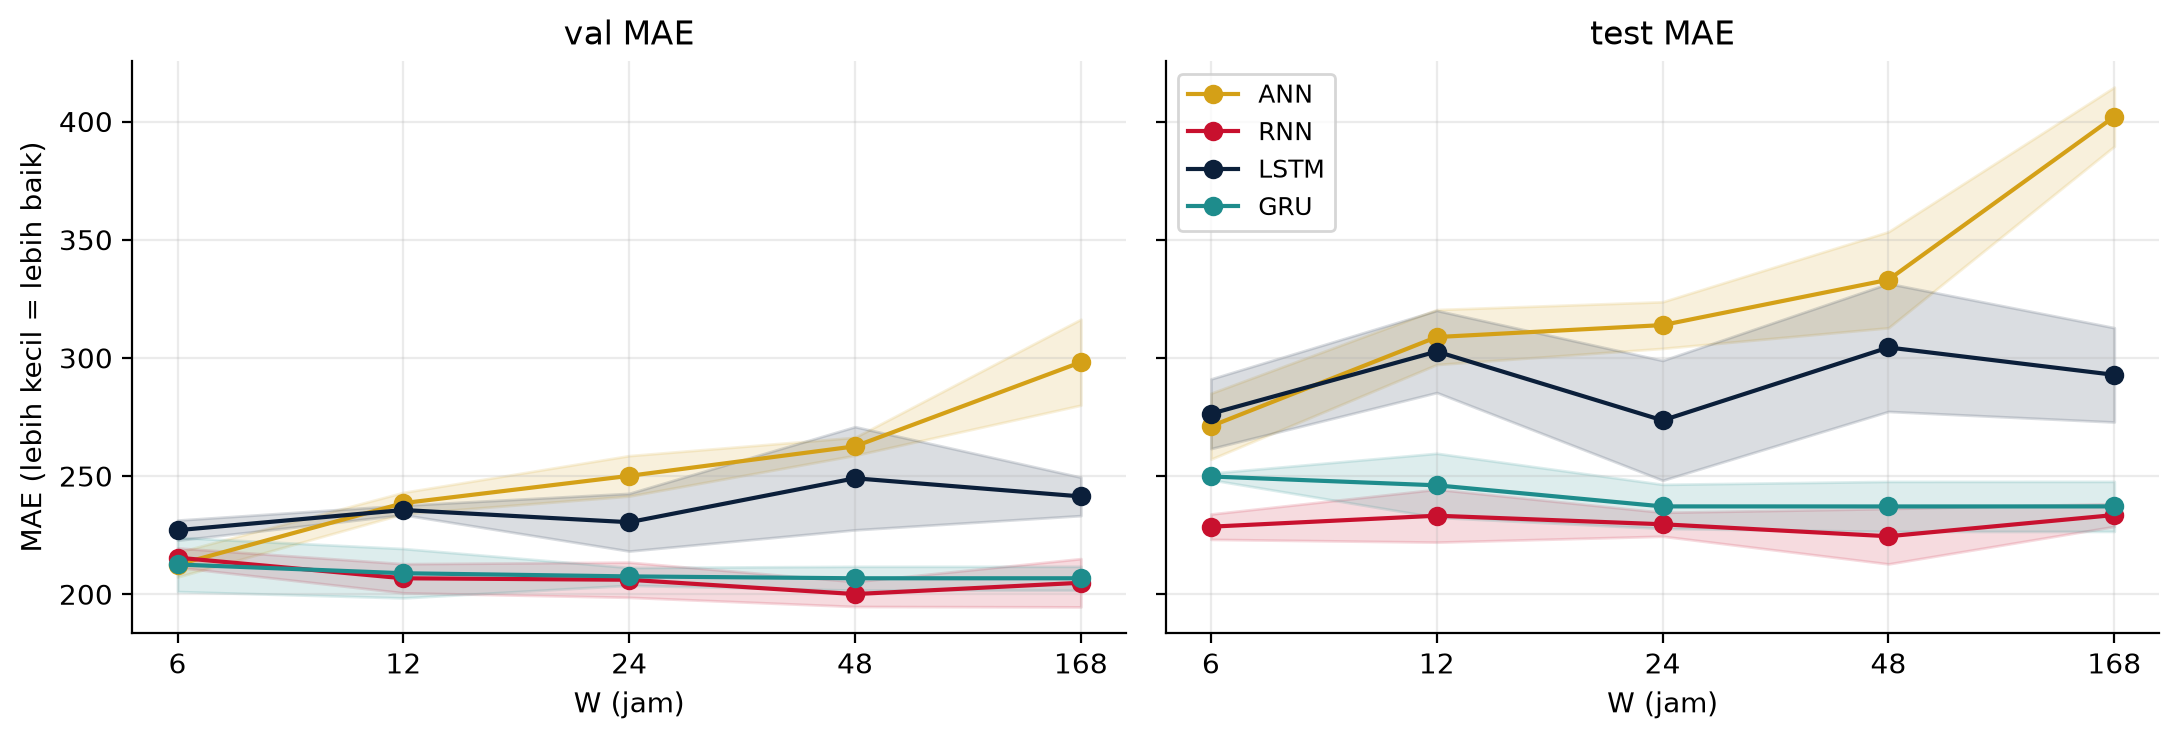
\includegraphics[width=\linewidth]{A1_W.png}\caption{A1: panjang jendela $W$}\end{subfigure}\hfill
\begin{subfigure}[t]{0.49\textwidth}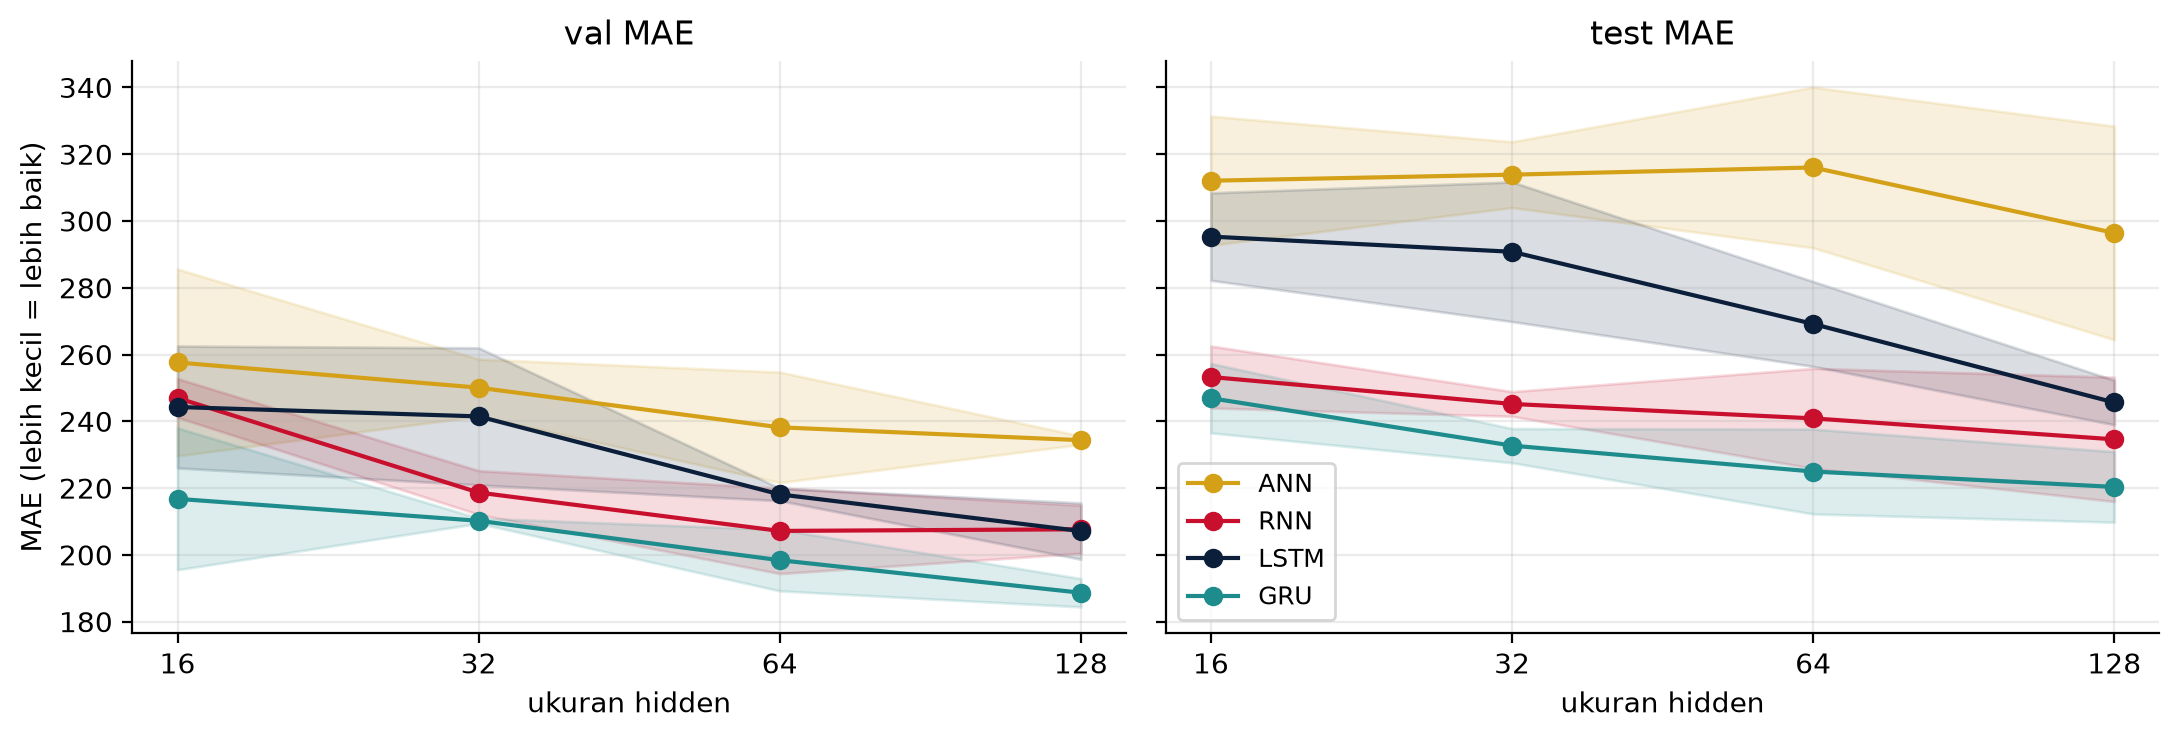
\includegraphics[width=\linewidth]{A2_hidden.png}\caption{A2: ukuran hidden}\end{subfigure}\\[4pt]
\begin{subfigure}[t]{0.49\textwidth}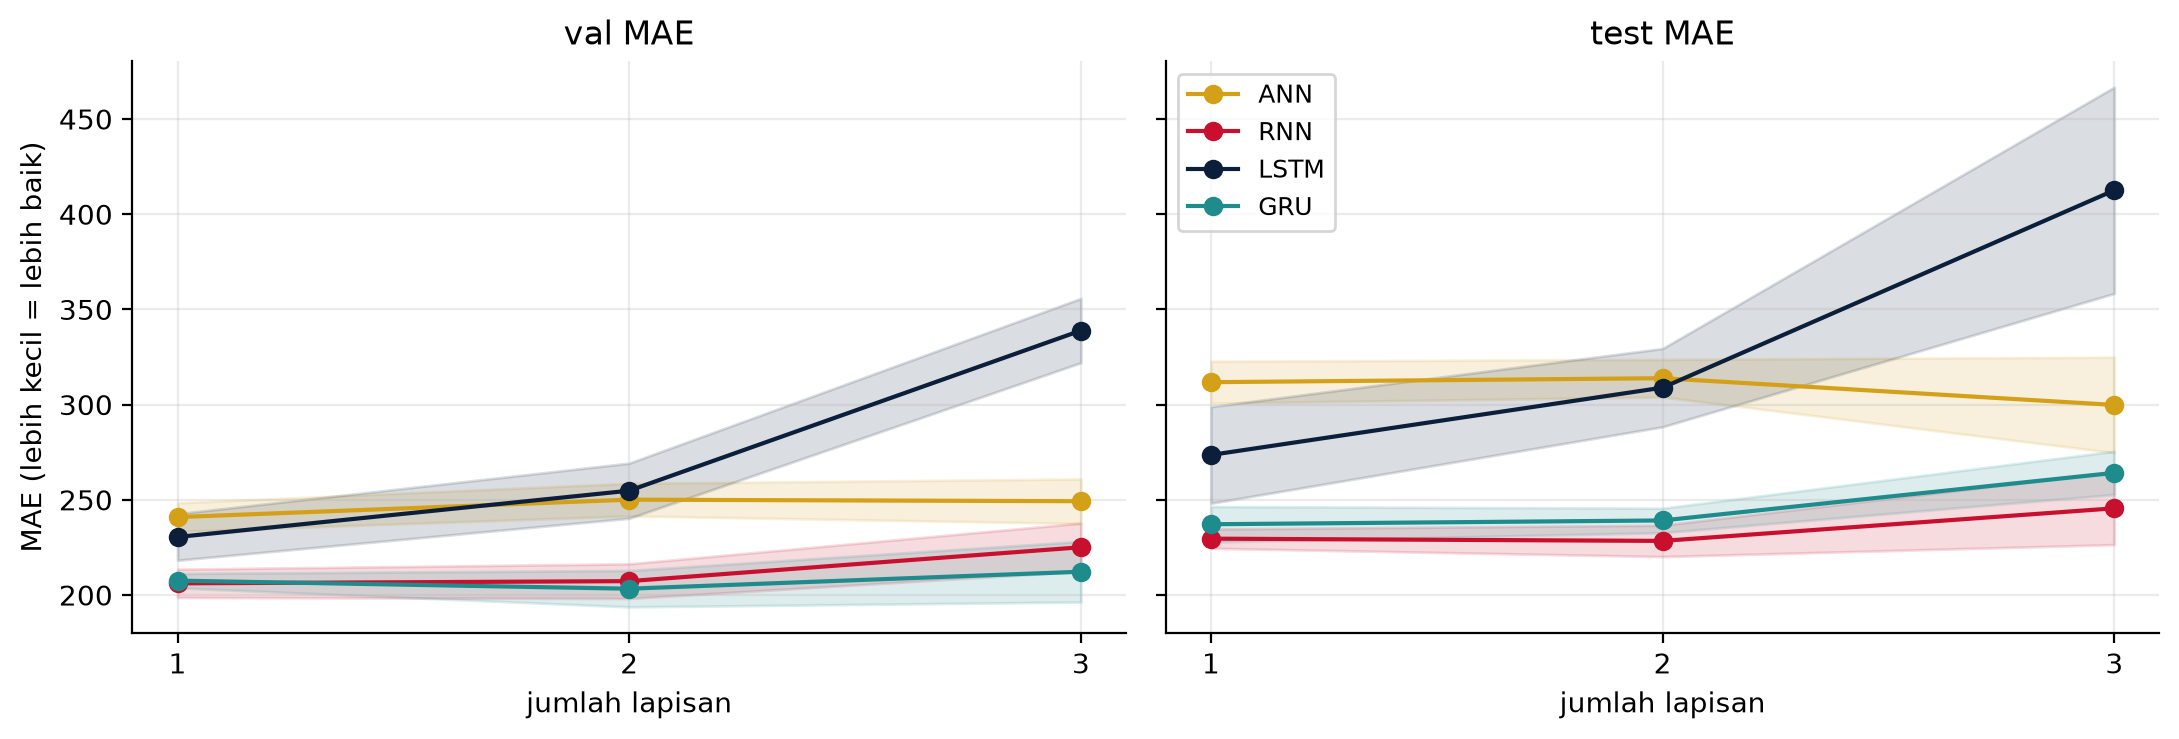
\includegraphics[width=\linewidth]{A3_layers.png}\caption{A3: jumlah lapisan}\end{subfigure}\hfill
\begin{subfigure}[t]{0.49\textwidth}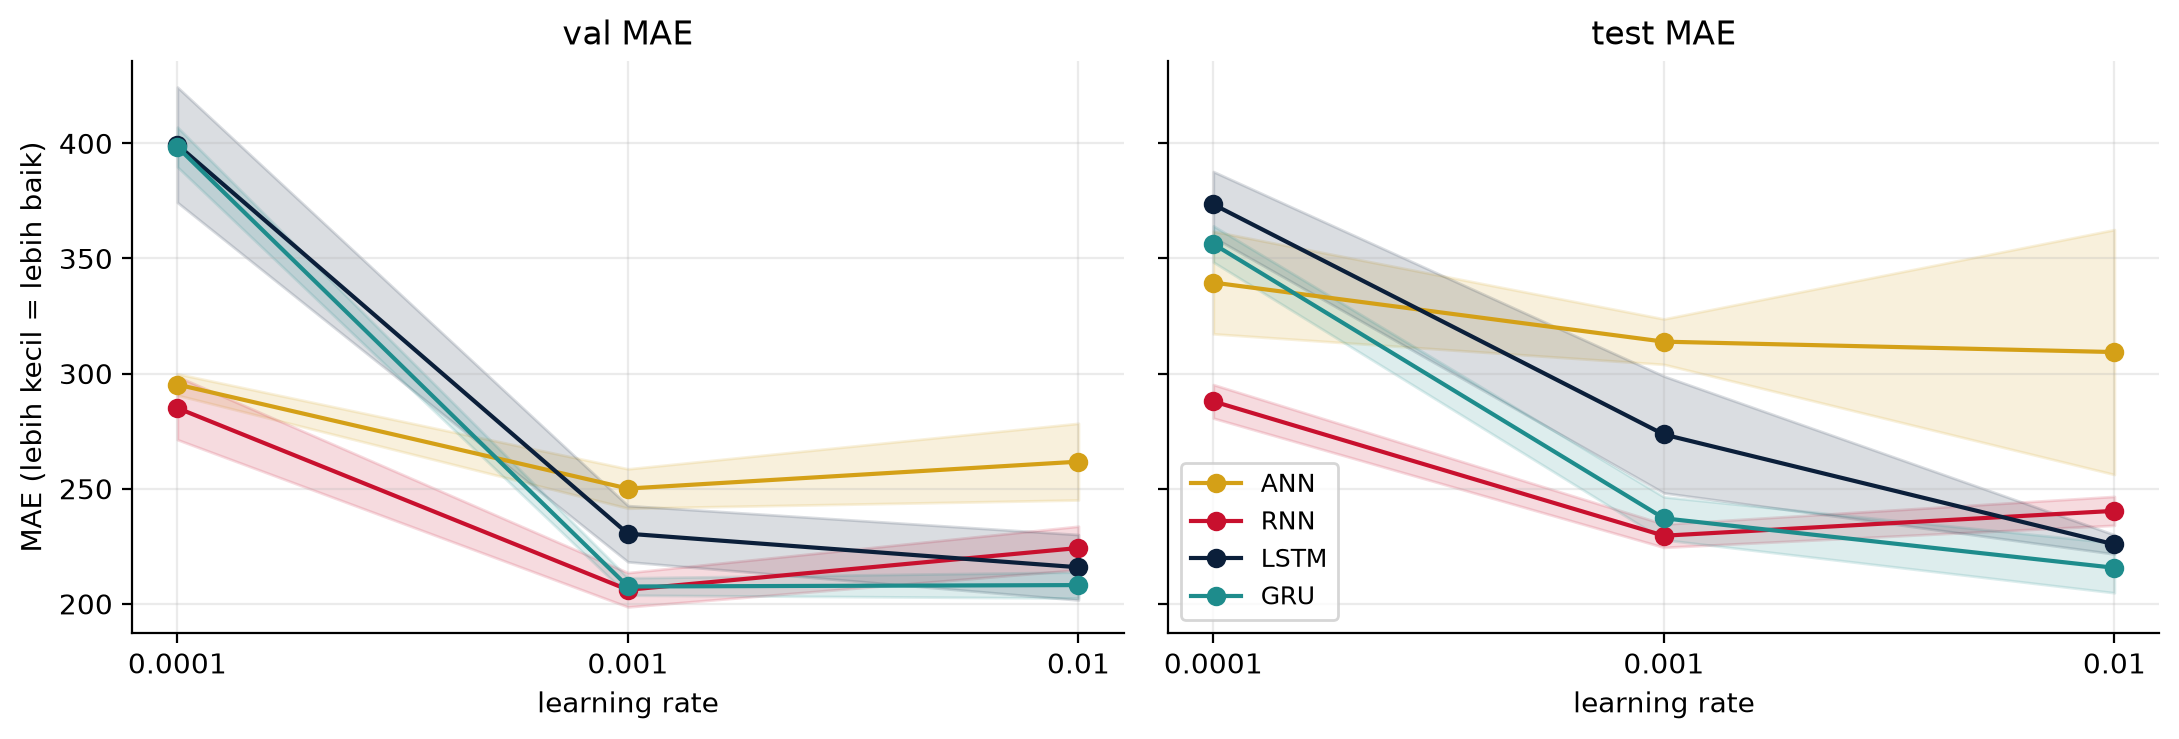
\includegraphics[width=\linewidth]{A4_lr.png}\caption{A4: \emph{learning rate}}\end{subfigure}\\[4pt]
\begin{subfigure}[t]{0.49\textwidth}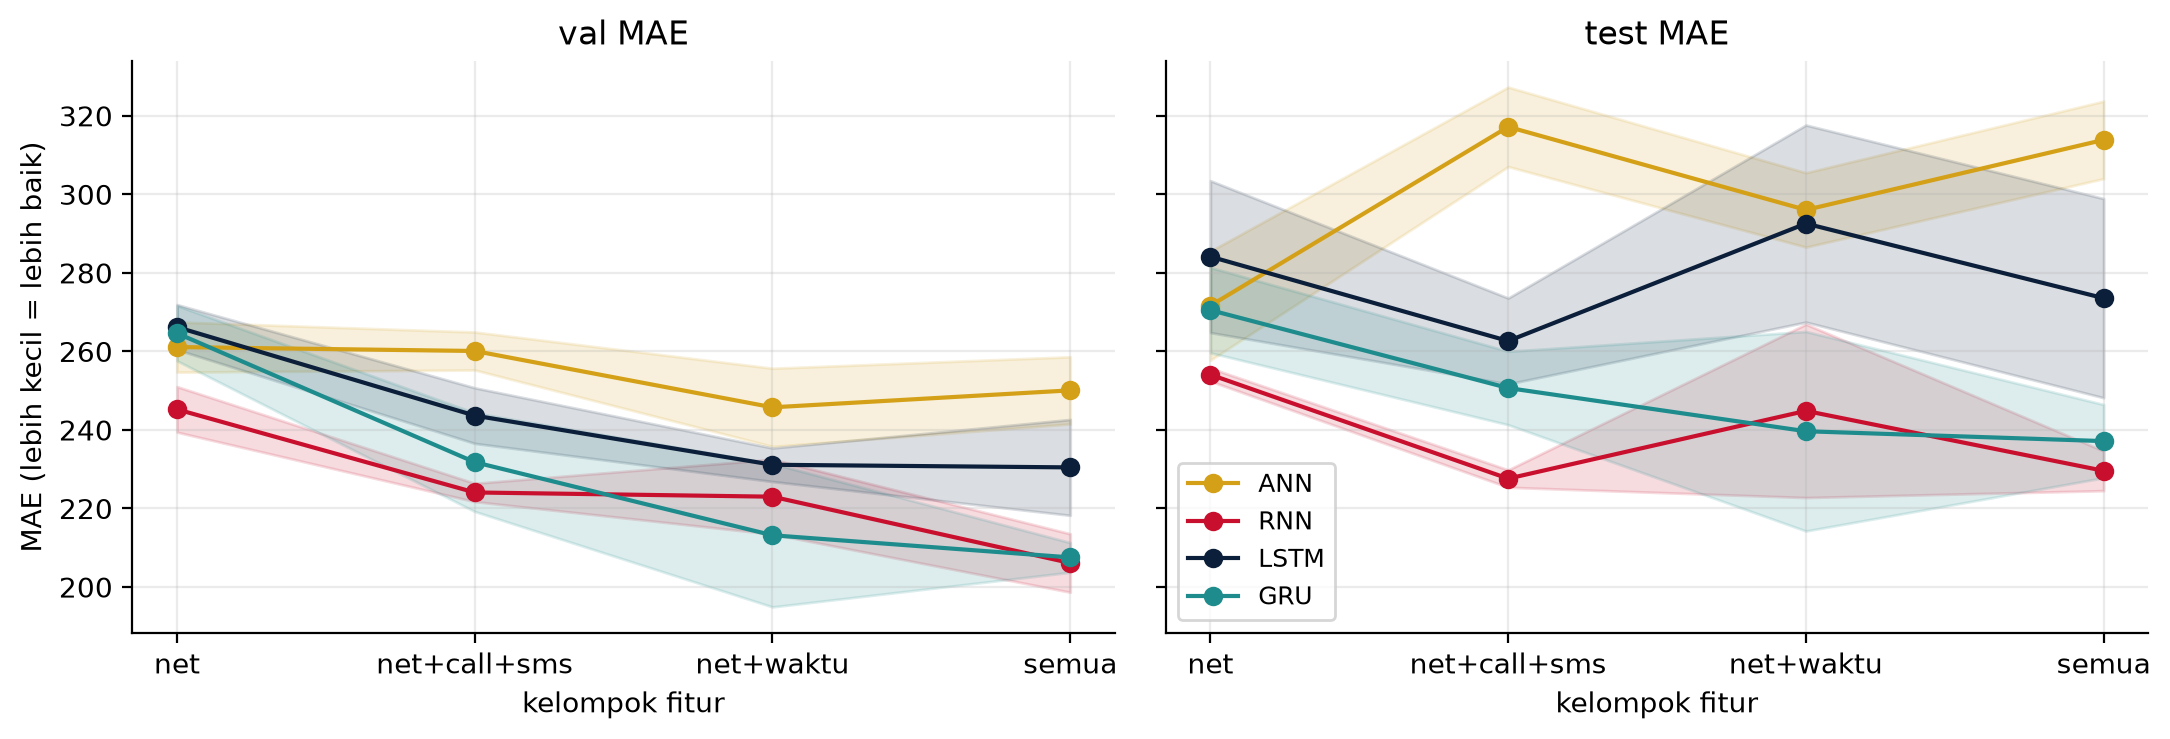
\includegraphics[width=\linewidth]{A5_fitur.png}\caption{A5: kelompok fitur}\end{subfigure}
\caption{Ablasi wajib. Setiap panel menunjukkan MAE validasi (kiri) dan MAE uji (kanan) sebagai rata-rata tiga seed dengan pita simpangan baku; lebih rendah lebih baik.}
\label{fig:ablasiA}
\end{figure*}

\textbf{A1, panjang jendela.} Jendela yang lebih panjang tidak selalu lebih baik (Gambar~\ref{fig:ablasiA}a, Tabel~\ref{tab:W}). MAE uji ANN naik dari 271,1 pada $W=6$ menjadi 402,0 pada $W=168$ karena jumlah parameternya tumbuh dari 2.465 menjadi 38.753 sementara data latih hanya 672 sampel, sehingga ANN cenderung \emph{overfit}. Model rekuren tidak mengalami hal itu karena parameternya tetap (5.305--5.578) dan bobotnya dipakai bersama di setiap langkah waktu. RNN dan GRU hampir tidak berubah (RNN 224--233, GRU 237--250), sedangkan LSTM berayun di kisaran 274--303.

\begin{table}[t]
\centering
\caption{Pengaruh Panjang Jendela $W$ terhadap MAE Uji (rata-rata $\pm$ simpangan baku, 3 seed)}
\label{tab:W}
\footnotesize
\setlength{\tabcolsep}{3pt}
\begin{tabular}{@{}rcccc@{}}
\toprule
$W$ (jam) & ANN & RNN & LSTM & GRU \\
\midrule
6   & $271{,}1\pm13{,}9$ & $228{,}6\pm5{,}4$  & $276{,}3\pm14{,}7$ & $249{,}8\pm1{,}4$ \\
24  & $313{,}9\pm9{,}9$  & $229{,}6\pm5{,}1$  & $273{,}6\pm25{,}4$ & $237{,}2\pm9{,}3$ \\
168 & $402{,}0\pm12{,}5$ & $233{,}5\pm4{,}8$  & $292{,}8\pm20{,}0$ & $237{,}2\pm10{,}6$ \\
\bottomrule
\end{tabular}
\end{table}

\textbf{A2, ukuran hidden.} Pada rentang yang diuji, model yang lebih besar justru membaik. GRU dengan hidden 128 mencapai MAE validasi 188,7 dan uji 220,3, terbaik dari seluruh percobaan ukuran, sedangkan LSTM membaik paling nyata, dari 295,3 ke 245,6 pada uji. Hal ini menunjukkan bahwa pada data sekecil ini kapasitas belum menjadi masalah selama model rekuren memakai bobot bersama; ANN hanya sedikit terbantu (312,1 menjadi 296,4). Perlu dicatat bahwa jumlah parameter tidak lagi setara, misalnya LSTM hidden 128 memiliki 70.273 parameter dibanding 17.665 pada RNN.

\textbf{A3, jumlah lapisan.} Menumpuk lapisan rekuren tidak membantu. Pada tiga lapisan, LSTM memburuk tajam (uji 412,6 dibanding 273,6 pada satu lapisan) dan lebih tidak stabil (simpangan baku 54,2), sedangkan RNN dan GRU hanya naik sedikit (245,5 dan 264,2). Epoch rata-rata model yang lebih dalam cenderung lebih sedikit (misalnya LSTM 168,7 menjadi 134,0 epoch), sehingga model dalam berhenti lebih cepat tetapi pada hasil yang lebih buruk, konsisten dengan kecenderungan \emph{overfit} dan sulitnya optimasi pada data kecil.

\textbf{A4, \emph{learning rate}.} Pada $10^{-4}$ seluruh model berhenti tepat di batas 300 epoch, artinya pelatihan terhenti karena \texttt{max\_epochs} sebelum konvergen; LSTM dan GRU paling terdampak (MAE validasi sekitar 399). Pada $10^{-2}$ pelatihan jauh lebih cepat (60--68 epoch) dan LSTM serta GRU justru terbaik di data uji (225,8 dan 215,7), tetapi RNN sedikit memburuk (240,4 dibanding 229,6) dan simpangan baku ANN membesar (53,2). Jadi nilai $10^{-3}$ adalah kompromi yang aman, sedangkan $10^{-2}$ menguntungkan gerbang LSTM/GRU.

\textbf{A5, kelompok fitur.} Informasi jam dan hari ternyata lebih berguna daripada trafik telepon/SMS bagi sebagian besar model pada validasi: MAE validasi RNN turun dari 245,2 (net) menjadi 206,1 (semua), dan GRU dari 264,6 menjadi 207,5. Pada data uji hasilnya lebih campuran; RNN terbaik dengan net+call+sms (227,6) sedangkan ANN terbaik dengan net saja (271,7). Pada validasi, penambahan fitur waktu membantu model rekuren lebih besar daripada ANN (GRU turun 264,6 menjadi 213,2; ANN 261,1 menjadi 245,8), tetapi pada data uji pengaruhnya tidak konsisten dan simpangan bakunya besar, sehingga kesimpulan tentang fitur waktu perlu diambil dengan hati-hati.

\subsection{Ablasi Pilihan}
\begin{figure}[t]
\centering
\begin{subfigure}[t]{\columnwidth}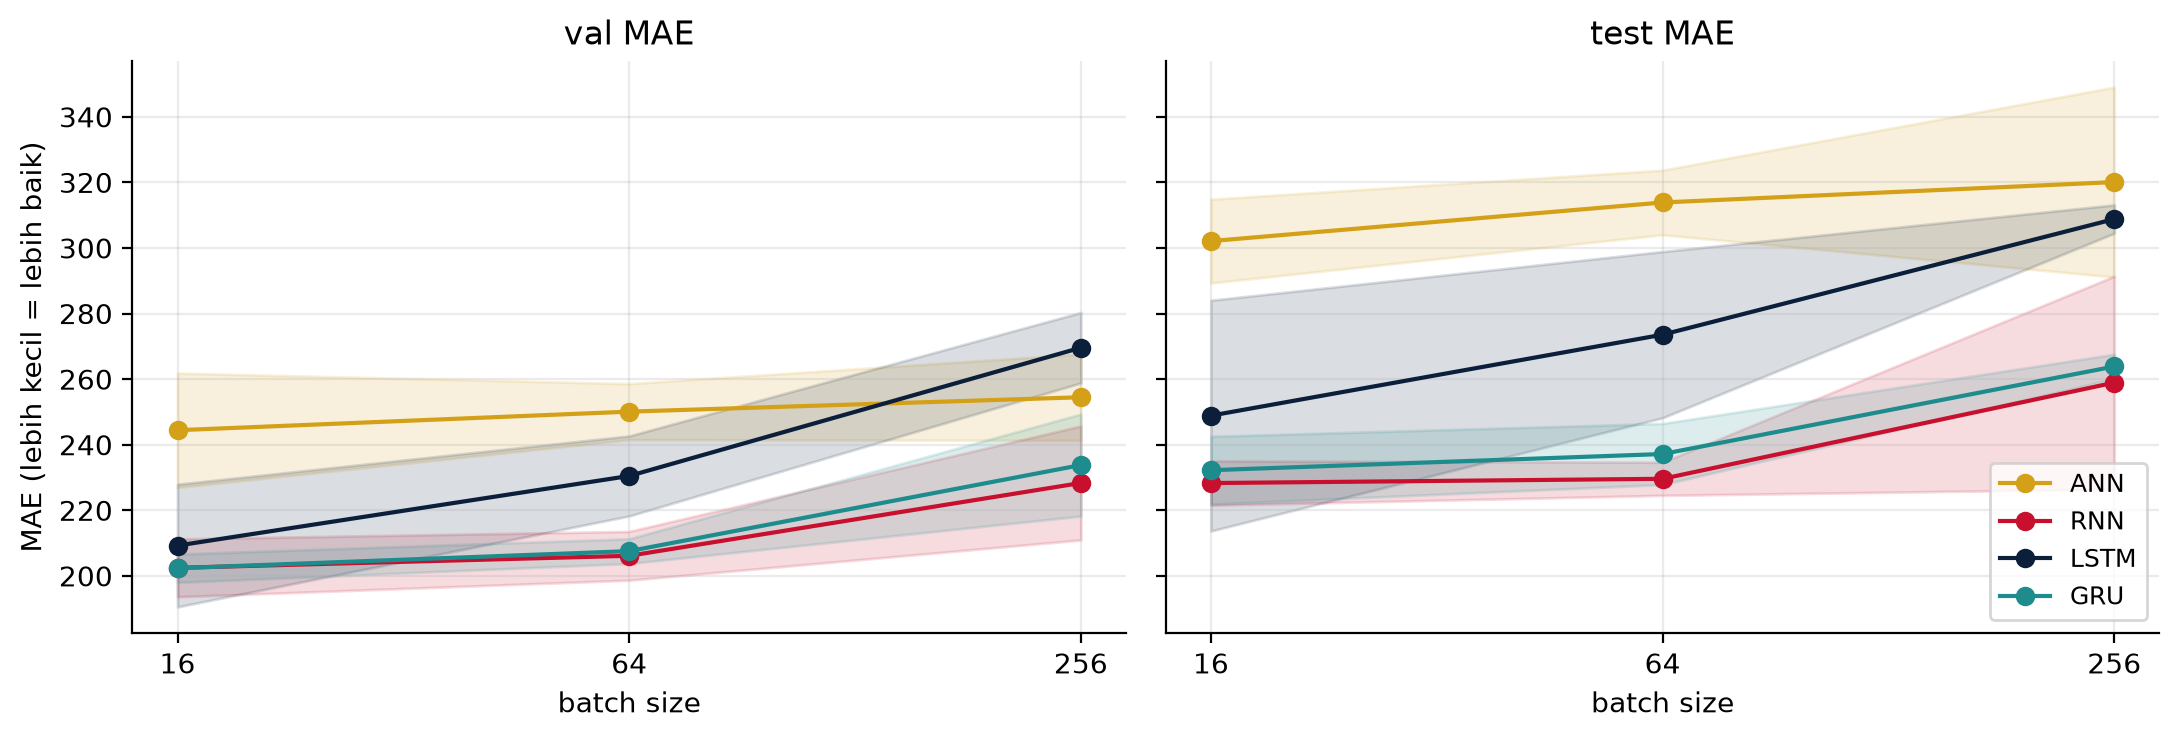
\includegraphics[width=\linewidth]{B1_batch.png}\caption{B1: \emph{batch size}}\end{subfigure}\\[3pt]
\begin{subfigure}[t]{\columnwidth}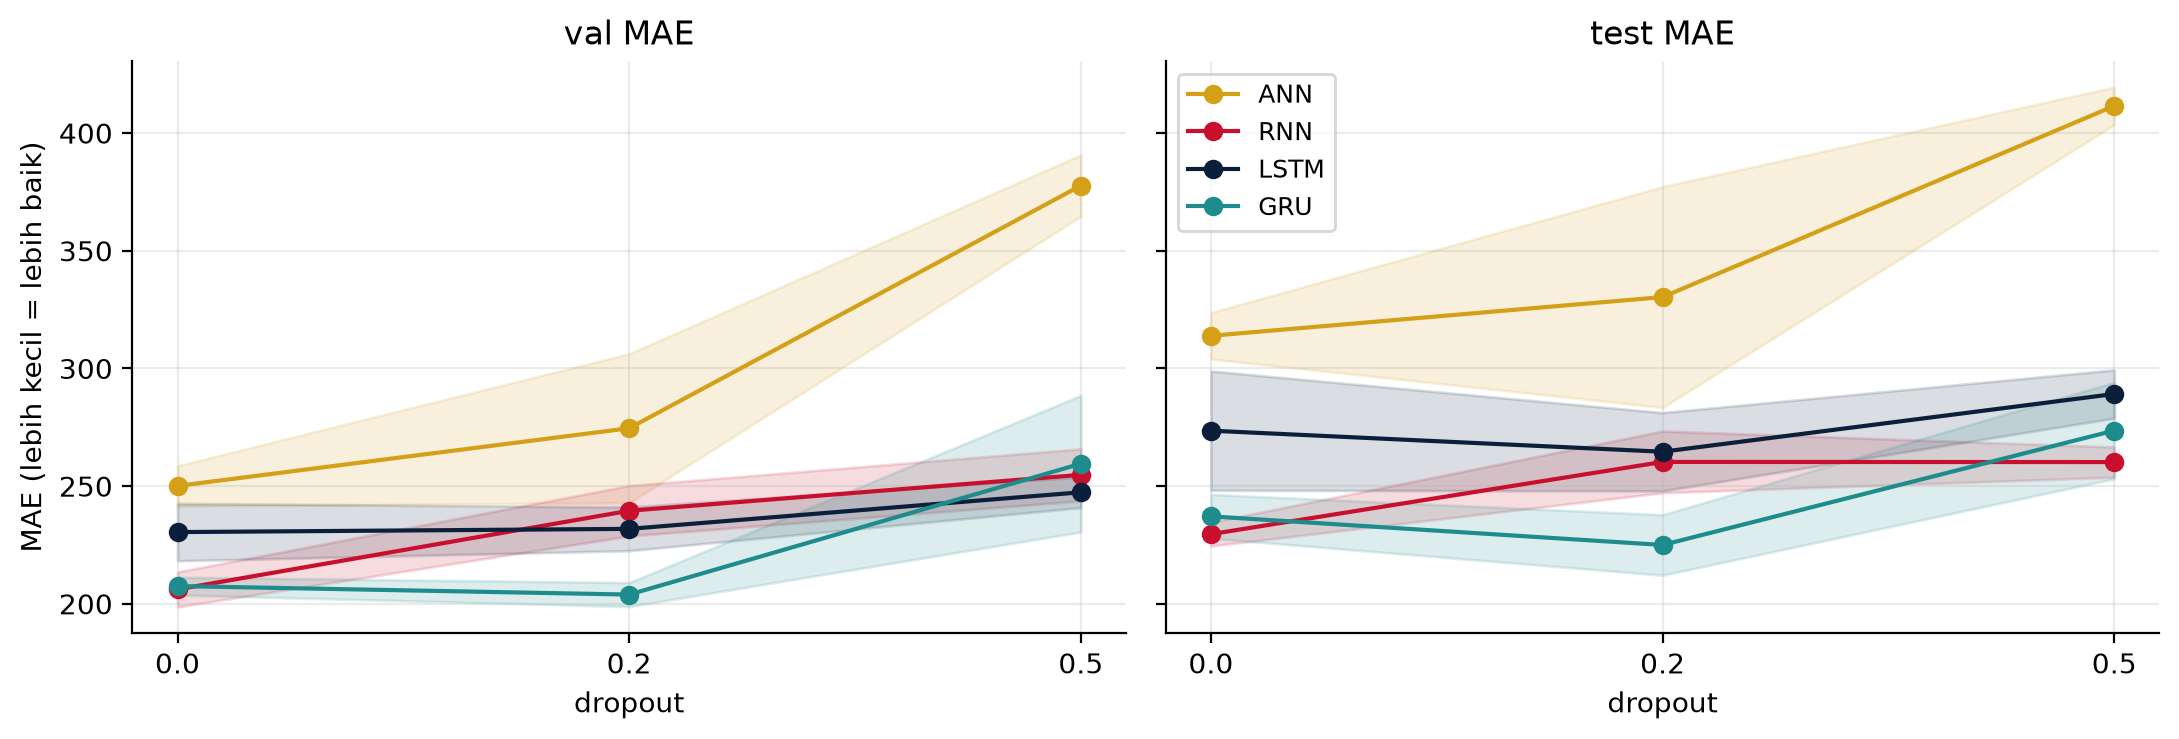
\includegraphics[width=\linewidth]{B2_dropout.png}\caption{B2: \emph{dropout}}\end{subfigure}\\[3pt]
\begin{subfigure}[t]{\columnwidth}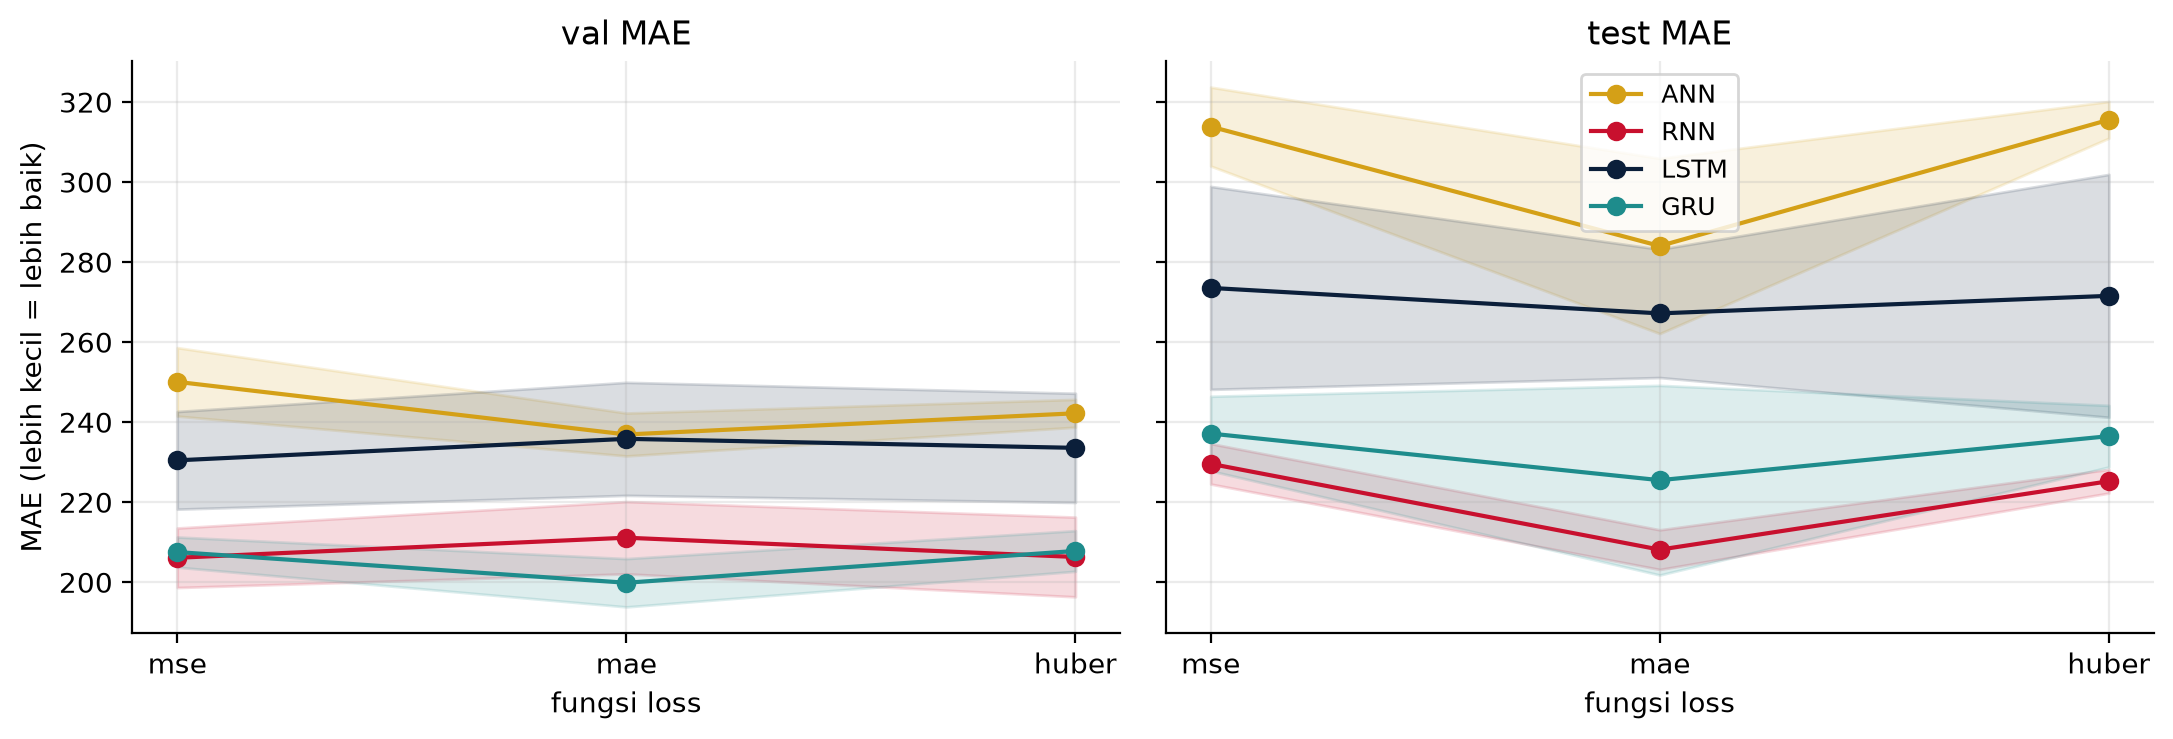
\includegraphics[width=\linewidth]{B4_loss.png}\caption{B4: fungsi \emph{loss}}\end{subfigure}\\[3pt]
\begin{subfigure}[t]{\columnwidth}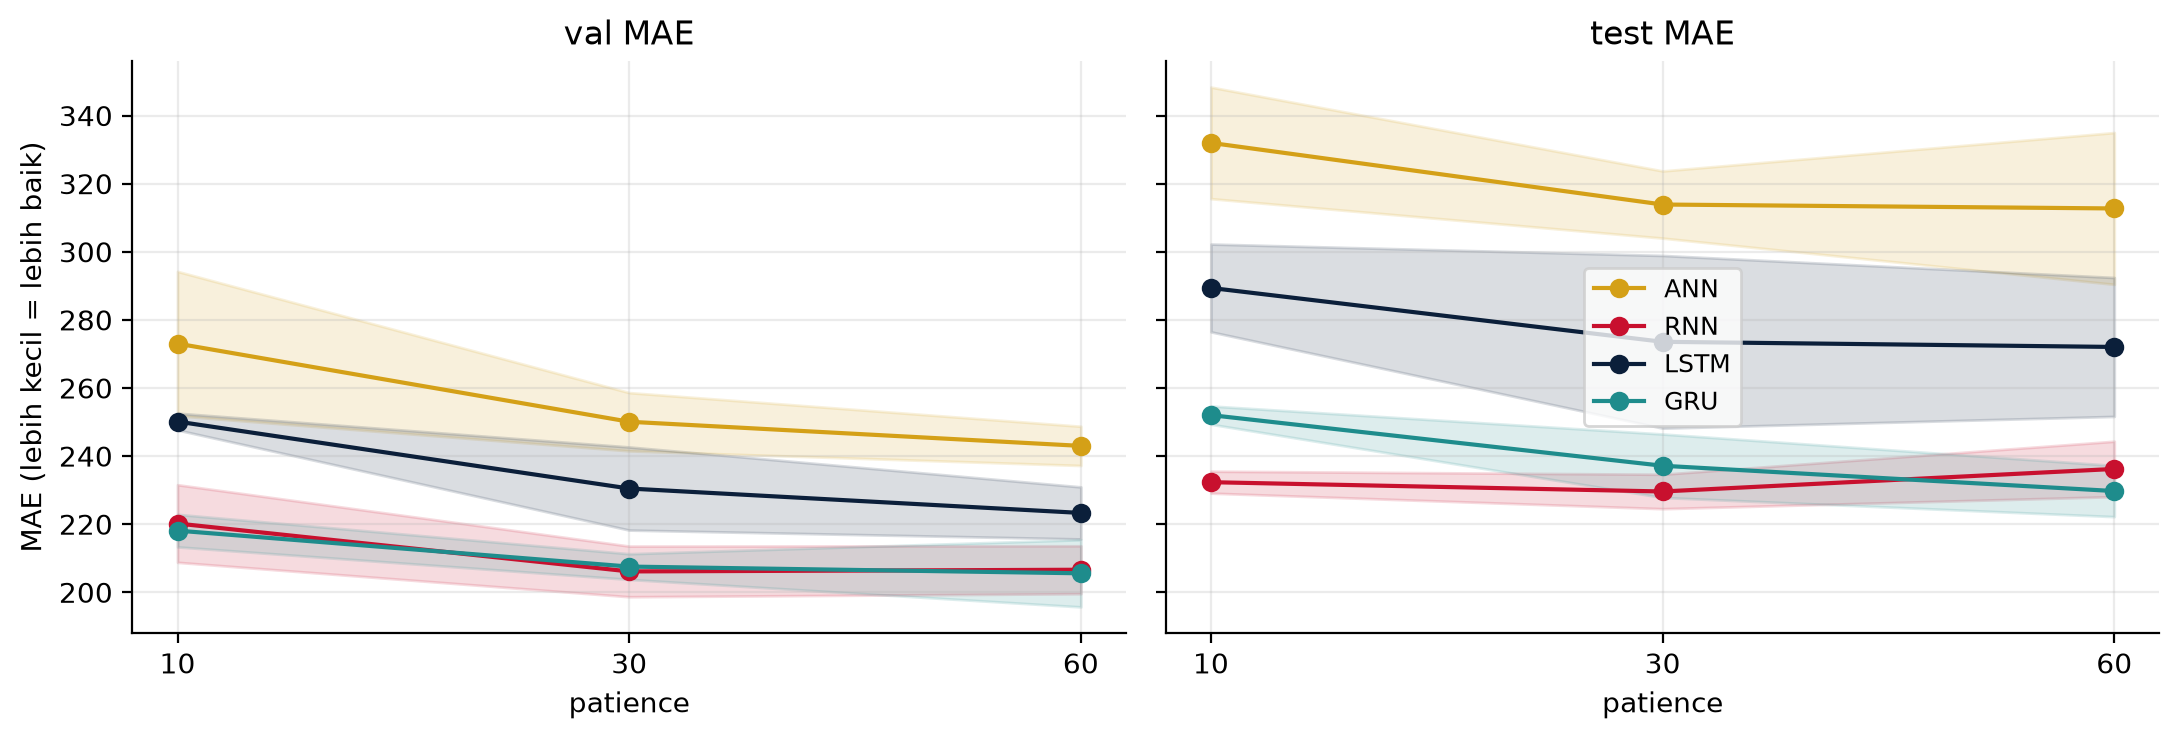
\includegraphics[width=\linewidth]{B5_patience.png}\caption{B5: \emph{patience}}\end{subfigure}
\caption{Ablasi pilihan (MAE validasi kiri, uji kanan).}
\label{fig:ablasiB}
\end{figure}

\textbf{B1, \emph{batch size}.} Batch kecil (16) terbaik untuk semua model, dan batch 256 terburuk (misalnya GRU uji 263,9 vs 232,2) sekaligus paling lama karena membutuhkan lebih banyak epoch (GRU mencapai batas 300). Dengan hanya 672 sampel, batch 256 berarti hanya tiga pembaruan per epoch.

\textbf{B2, \emph{dropout}.} Regularisasi tidak membantu pada data sekecil ini. ANN memburuk drastis pada $p=0{,}5$ (uji 411,6 dibanding 313,9), sementara hanya GRU yang sedikit membaik pada $p=0{,}2$ (MAE validasi 203,9 dan uji 225,0), sehingga hipotesis awal kami sebagian besar terkonfirmasi.

\textbf{B4, \emph{loss}.} Loss MAE menurunkan MAE uji pada keempat model dibanding mse (RNN 229,6 menjadi 208,2; ANN 313,9 menjadi 284,0), selaras dengan metrik evaluasinya. Namun berdasarkan MAE validasi, RNN dan LSTM tetap memilih mse, sehingga pilihan berbasis validasi melewatkan keuntungan di data uji pada RNN.

\textbf{B5, \emph{patience}.} Patience 10 menghentikan pelatihan terlalu dini (ANN 61 epoch, uji 332,0), sedangkan 30 dan 60 hasilnya mirip untuk RNN dan GRU. LSTM dan ANN masih membaik pada 60.

Tabel~\ref{tab:best} merangkum nilai terbaik tiap faktor menurut MAE validasi.

\begin{table}[t]
\centering
\caption{Nilai Terbaik per Faktor Menurut MAE Validasi}
\label{tab:best}
\footnotesize
\setlength{\tabcolsep}{3pt}
\begin{tabular}{@{}lcccc@{}}
\toprule
Faktor & ANN & RNN & LSTM & GRU \\
\midrule
$W$ (jam)         & 6    & 48  & 6    & 48 \\
Hidden            & 128  & 64  & 128  & 128 \\
Lapisan           & 1    & 1   & 1    & 2 \\
\emph{Learning rate} & $10^{-3}$ & $10^{-3}$ & $10^{-2}$ & $10^{-3}$ \\
Fitur             & net+waktu & semua & semua & semua \\
\emph{Batch size} & 16   & 16  & 16   & 16 \\
\emph{Dropout}    & 0    & 0   & 0    & 0,2 \\
\emph{Loss}       & mae  & mse & mse  & mae \\
\emph{Patience}   & 60   & 30  & 60   & 60 \\
\bottomrule
\end{tabular}
\end{table}

\subsection{Konfigurasi Terbaik}
Nilai-nilai terbaik per faktor digabungkan menjadi satu konfigurasi per model dan dilatih ulang dengan tiga seed (Tabel~\ref{tab:C}, Gambar~\ref{fig:C}). Konfigurasinya adalah ANN: $W=6$, hidden 128, satu lapisan, fitur net+waktu, batch 16, loss mae, patience 60; RNN: $W=48$, batch 16; LSTM: $W=6$, hidden 128, \emph{learning rate} $10^{-2}$, batch 16, patience 60; GRU: $W=48$, hidden 128, dua lapisan, batch 16, \emph{dropout} 0,2, loss mae, patience 60. Seluruh model membaik pada pekan uji maupun Natal terhadap acuan. Peningkatan terbesar dialami ANN (MAE uji turun 18,8\%) dan LSTM (10,5\%), sedangkan RNN nyaris tidak berubah (1,4\%) karena acuannya sudah dekat dengan optimum. MAPE uji juga turun pada semua model (misalnya ANN 11,7\% menjadi 8,5\% dan GRU 8,0\% menjadi 7,1\%). GRU terbaik (221,9) memiliki 151.809 parameter, sekitar 29 kali lipat RNN dengan MAE yang hanya sedikit berbeda (226,3 dengan 5.305 parameter), sehingga dari sisi efisiensi RNN sangat kompetitif. Terhadap baseline naif terbaik (468), GRU dan RNN menurunkan MAE sekitar 52\%.

\begin{table}[t]
\centering
\caption{Acuan vs Terbaik, Duomo (MAE rata-rata $\pm$ simpangan baku, 3 seed)}
\label{tab:C}
\footnotesize
\setlength{\tabcolsep}{2.5pt}
\begin{tabular}{@{}llrccc@{}}
\toprule
Model & Konfig. & Param. & MAE uji & MAPE uji (\%) & MAE Natal \\
\midrule
ANN  & acuan  & 6.497   & $313{,}9\pm9{,}9$  & 11,7 & $675{,}7\pm44{,}6$ \\
     & terbaik& 4.097   & $254{,}9\pm9{,}0$  & 8,5  & $569{,}9\pm75{,}1$ \\
RNN  & acuan  & 5.305   & $229{,}6\pm5{,}1$  & 8,5  & $421{,}2\pm2{,}4$ \\
     & terbaik& 5.305   & $226{,}3\pm4{,}9$  & 8,2  & $385{,}4\pm13{,}8$ \\
LSTM & acuan  & 5.578   & $273{,}6\pm25{,}4$ & 9,1  & $586{,}0\pm56{,}8$ \\
     & terbaik& 70.273  & $245{,}0\pm11{,}6$ & 8,4  & $469{,}5\pm7{,}8$ \\
GRU  & acuan  & 5.397   & $237{,}2\pm9{,}3$  & 8,0  & $468{,}2\pm21{,}8$ \\
     & terbaik& 151.809 & $221{,}9\pm14{,}3$ & 7,1  & $454{,}8\pm18{,}1$ \\
\bottomrule
\end{tabular}
\end{table}

\begin{figure}[t]
\centering
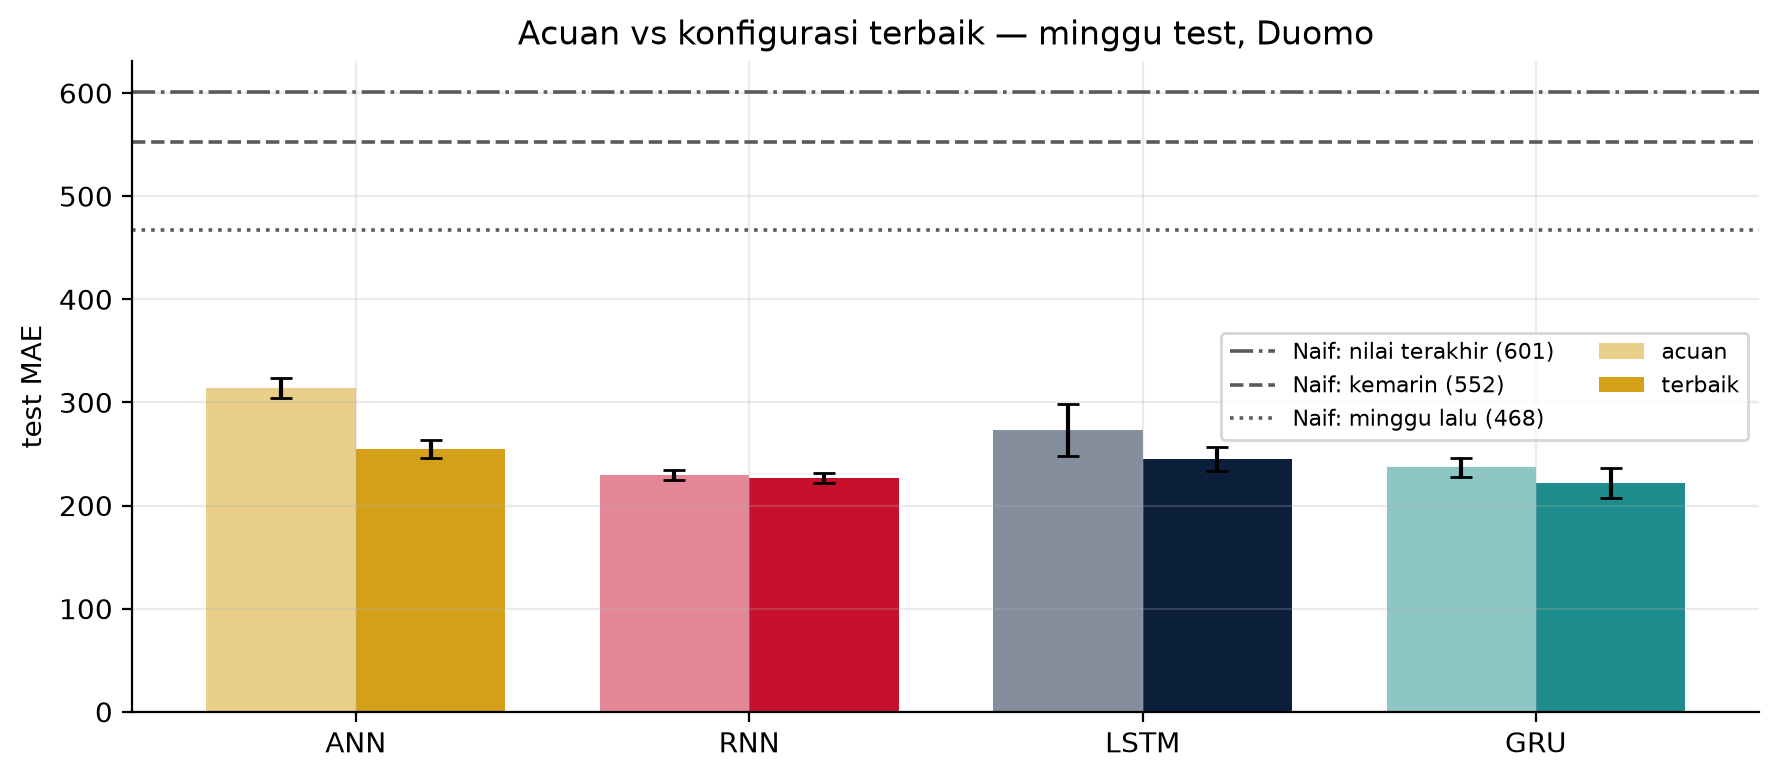
\includegraphics[width=\columnwidth]{C_terbaik_vs_acuan.png}
\caption{MAE uji acuan (warna terang) dan konfigurasi terbaik (warna gelap) pada minggu uji Duomo, dibandingkan tiga baseline naif (garis putus-putus).}
\label{fig:C}
\end{figure}

\subsection{Uji Generalisasi}
Konfigurasi acuan dan terbaik dari Duomo dilatih ulang tanpa diubah di Universitas Bicocca (kode lokasi 7; Tabel~\ref{tab:D}). Sebagaimana terlihat pada Gambar~\ref{fig:pola}, deret Bicocca tidak stasioner: levelnya menurun tajam sepanjang periode, sehingga model yang dilatih pada minggu-minggu awal menghadapi data uji dan Natal dengan level yang jauh lebih rendah. Baseline naif di Bicocca memberi MAE uji 105,5 (nilai terakhir), 186,4 (kemarin), dan 63,8 (pekan lalu). Seluruh model mengalahkan baseline terbaik pada pekan uji dengan MAE 42,8--52,9; konfigurasi terbaik LSTM dan GRU (42,8 dan 43,9) berada sekitar 33\% dan 31\% di bawah baseline pekan lalu.

Konfigurasi terbaik dari Duomo tetap berguna di lokasi baru. MAE uji turun untuk LSTM (52,9 menjadi 42,8), GRU (50,5 menjadi 43,9), dan ANN (50,8 menjadi 46,2), sedangkan RNN nyaris tidak berubah (47,8 menjadi 47,2); MAPE uji turun dari kisaran 14--16\% menjadi 11,5--14,4\%. Urutan model berbeda dari Duomo: pada acuan RNN terbaik (47,8) dan LSTM terburuk (52,9), tetapi pada konfigurasi terbaik LSTM (42,8) dan GRU (43,9) berada di depan, sedangkan RNN (47,2) tertinggal. Namun selisih antar model selain peningkatan LSTM berada dalam kisaran simpangan baku (2--5), sehingga urutan itu tidak boleh ditafsirkan terlalu kuat.

Pada pekan Natal hasilnya jauh berbeda. Baseline nilai terakhir (23,1) dan nilai kemarin (48,6) mengalahkan semua model (MAE 139,5--285,6), dan hanya baseline pekan lalu (355,2) yang lebih buruk daripada model. Konfigurasi terbaik tetap menurunkan MAE Natal sebesar 18\% (RNN) hingga 50\% (ANN), tetapi galatnya masih berkali-kali lipat baseline sederhana. Hal ini konsisten dengan penurunan level aktivitas yang sangat tajam pada akhir tahun, yang tidak pernah dilihat model saat pelatihan.

\begin{table}[t]
\centering
\caption{Generalisasi ke Universitas Bicocca: MAE Uji (rata-rata $\pm$ simpangan baku, 3 seed) dan MAE Natal (rata-rata)}
\label{tab:D}
\footnotesize
\setlength{\tabcolsep}{3pt}
\begin{tabular}{@{}lcccc@{}}
\toprule
 & \multicolumn{2}{c}{MAE uji} & \multicolumn{2}{c}{MAE Natal} \\
\cmidrule(lr){2-3}\cmidrule(lr){4-5}
Model & acuan & terbaik & acuan & terbaik \\
\midrule
ANN  & $50{,}8\pm2{,}4$ & $46{,}2\pm3{,}5$ & 285,6 & 143,8 \\
RNN  & $47{,}8\pm2{,}9$ & $47{,}2\pm5{,}3$ & 169,2 & 139,5 \\
LSTM & $52{,}9\pm2{,}6$ & $42{,}8\pm2{,}1$ & 246,2 & 153,8 \\
GRU  & $50{,}5\pm3{,}5$ & $43{,}9\pm2{,}5$ & 255,2 & 169,4 \\
\midrule
\multicolumn{5}{@{}l}{\emph{Baseline naif (uji / Natal)}} \\
Nilai terakhir & \multicolumn{2}{c}{105,5} & \multicolumn{2}{c}{23,1} \\
Kemarin        & \multicolumn{2}{c}{186,4} & \multicolumn{2}{c}{48,6} \\
Pekan lalu     & \multicolumn{2}{c}{63,8}  & \multicolumn{2}{c}{355,2} \\
\bottomrule
\end{tabular}
\end{table}

\section{Pembahasan}
Hasil menunjukkan bahwa pada data sekecil ini (satu kota, empat minggu latih, satu kali pembagian waktu) arsitektur bukan satu-satunya penentu; pilihan hiperparameter sering sama pentingnya. Faktor yang paling berpengaruh adalah \emph{learning rate} (kegagalan konvergen pada $10^{-4}$), panjang jendela untuk ANN, jumlah lapisan untuk LSTM, dan \emph{dropout} berlebih untuk ANN. Faktor yang relatif tidak peka bagi model rekuren adalah panjang jendela dan fitur waktu. Penjelasan yang konsisten adalah bahwa ANN membayar setiap tambahan langkah masukan dengan parameter baru, sedangkan model rekuren memakai bobot yang sama di tiap langkah.

Beberapa batasan perlu diakui. Pertama, tiga seed menghasilkan simpangan baku yang cukup besar pada beberapa konfigurasi (misalnya LSTM 25,4 pada acuan di Duomo), sehingga selisih kecil antar model, seperti RNN dan GRU, belum tentu bermakna. Kedua, ablasi mengubah satu faktor setiap kali; interaksi antar faktor baru diuji sekali saat konfigurasi terbaik digabungkan, dan penggabungan itu tidak selalu memberi hasil terbaik karena pemilihan memakai validasi (contohnya \emph{loss} MAE pada RNN). Ketiga, satu kota, satu periode, dan satu horizon (satu jam) membatasi klaim generalisasi; hasil di Bicocca memperlihatkan bahwa konfigurasi terbaik di Duomo masih membantu pada pekan uji tetapi urutan modelnya berubah, dan bahwa pekan Natal pada deret yang tidak stasioner tetap sulit bagi semua model dibanding baseline sederhana.

\section{Kesimpulan}
GRU dan RNN paling akurat di Duomo (MAE uji sekitar 222 dan 226), sekitar 52\% di bawah baseline naif terbaik, dengan RNN jauh lebih ringan. ANN paling sensitif terhadap panjang jendela dan \emph{dropout}, LSTM terhadap jumlah lapisan, dan semua model terhadap \emph{learning rate} yang terlalu kecil. Di Universitas Bicocca, konfigurasi terbaik dari Duomo memperbaiki LSTM, GRU, dan ANN pada pekan uji dan semua model mengalahkan baseline naif terbaik, tetapi urutan model berubah dan pada pekan Natal baseline nilai terakhir dan kemarin mengalahkan semua model.

\section*{Kontribusi Anggota}
\begin{tabular}{@{}ll@{}}
Ade Raka Maulana & Semua tugas \\
\end{tabular}

\section*{Pernyataan Penggunaan AI}
Claude (Anthropic) digunakan untuk membantu menyusun draf laporan LaTeX ini dari hasil run notebook dan Seluruh angka berasal dari run saya sendiri.

\section*{Kode dan Data}
Kode, notebook beserta output, dan seluruh hasil run tersedia di \url{https://github.com/rkaatxt/Tugas-AI.git}.

\bibliographystyle{IEEEtran}
\bibliography{references}

\end{document}